% ============================================================
% ปกหน้าตำราวิชาการมาตรฐานสากล (Academic Book Cover Architect)
% สไตล์เปิดโปร่ง ไร้กล่อง ไร้กรอบ พร้อมสัญลักษณ์ AI \& Deep Learning
% มหาวิทยาลัยราชภัฏรำไพพรรณี
% ============================================================
\thispagestyle{empty}
\begin{titlepage}
\begingroup
\setlength{\XeTeXlinebreakskip}{0pt}
\begin{tikzpicture}[remember picture, overlay]
    % 1. ภาพอาร์ตเวิร์ก 3D Pixar Semi-realistics แบบ Full-Bleed 100%
    \node[anchor=center, inner sep=0pt] at (current page.center) {
        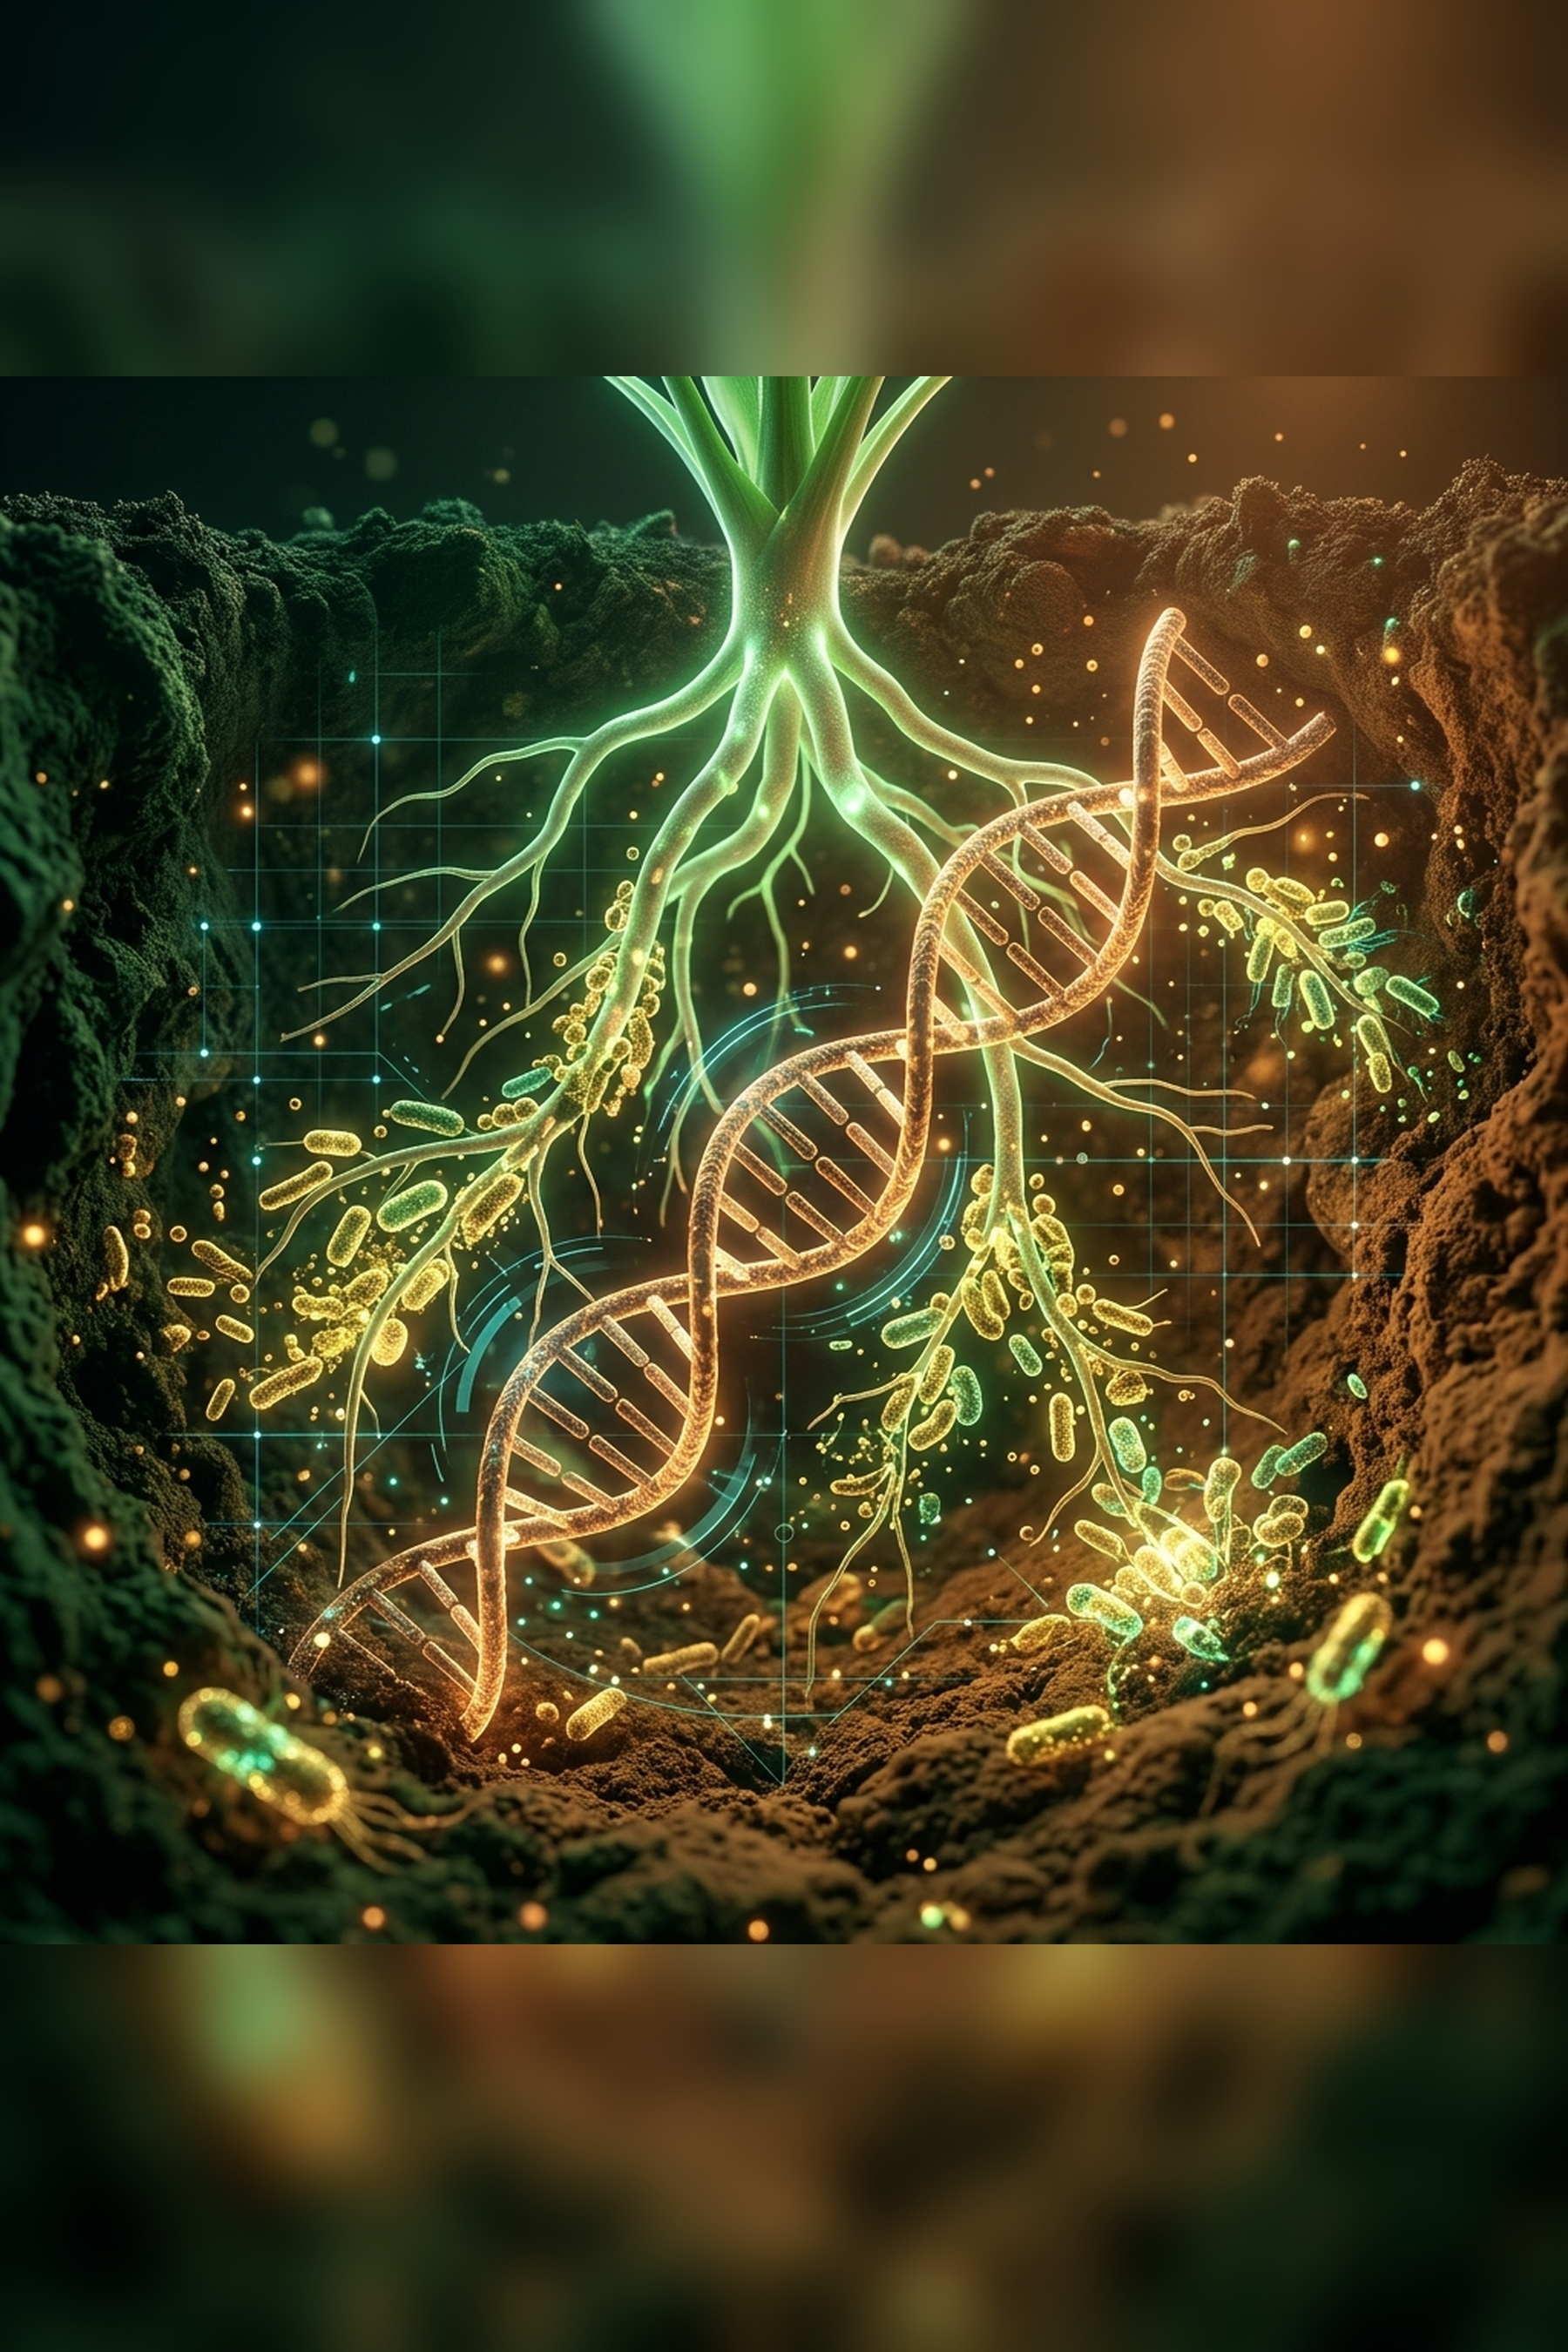
\includegraphics[width=\paperwidth, height=\paperheight]{assets/agri_cover_pixar_2x3.jpg}
    };

    % กำหนดสีสันสดใสระดับพรีเมียม (Curated Vibrant Palette)
    \definecolor{goldtitle}{RGB}{245, 195, 65}
    \definecolor{emeraldtitle}{RGB}{60, 230, 160}
    \definecolor{cyantitle}{RGB}{50, 220, 245}
    \definecolor{warmyellow}{RGB}{255, 235, 100}

    % ============================================================
    % สัญลักษณ์ AI / DEEP LEARNING (Header Neural Network Insignia)
    % ============================================================
    \begin{scope}[shift={([yshift=-0.60cm]current page.north)}]
        % Shadow layer
        \begin{scope}[shift={(0.6pt, -0.6pt)}]
            \foreach \ya in {-0.24, 0, 0.24} {
                \foreach \yb in {-0.34, -0.11, 0.11, 0.34} {
                    \draw[black!95, line width=0.5pt] (-2.2, \ya) -- (-1.8, \yb);
                }
            }
            \foreach \yb in {-0.34, -0.11, 0.11, 0.34} {
                \foreach \yc in {-0.17, 0.17} {
                    \draw[black!95, line width=0.5pt] (-1.8, \yb) -- (-1.4, \yc);
                }
            }
            \node[right, font=\fontsize{7pt}{8.5pt}\selectfont\bfseries, text=black!95] at (-1.25, 0) {ARTIFICIAL INTELLIGENCE \& DEEP LEARNING ARCHITECTURE};
        \end{scope}
        % Foreground layer
        \foreach \ya in {-0.24, 0, 0.24} {
            \foreach \yb in {-0.34, -0.11, 0.11, 0.34} {
                \draw[emeraldtitle!75, line width=0.4pt] (-2.2, \ya) -- (-1.8, \yb);
            }
        }
        \foreach \yb in {-0.34, -0.11, 0.11, 0.34} {
            \foreach \yc in {-0.17, 0.17} {
                \draw[goldtitle!75, line width=0.4pt] (-1.8, \yb) -- (-1.4, \yc);
            }
        }
        \foreach \ya in {-0.24, 0, 0.24} {
            \fill[emeraldtitle] (-2.2, \ya) circle (1.8pt);
            \draw[white, line width=0.3pt] (-2.2, \ya) circle (1.8pt);
        }
        \foreach \yb in {-0.34, -0.11, 0.11, 0.34} {
            \fill[emeraldtitle] (-1.8, \yb) circle (2pt);
            \draw[white, line width=0.3pt] (-1.8, \yb) circle (2pt);
        }
        \foreach \yc in {-0.17, 0.17} {
            \fill[goldtitle] (-1.4, \yc) circle (2.2pt);
            \draw[white, line width=0.3pt] (-1.4, \yc) circle (2.2pt);
        }
        \node[right, font=\fontsize{7pt}{8.5pt}\selectfont\bfseries, text=white] at (-1.25, 0) {ARTIFICIAL INTELLIGENCE \color{emeraldtitle}\&\ \color{goldtitle}DEEP LEARNING ARCHITECTURE};
    \end{scope}

    % ============================================================
    % 2. UPPER ZONE: ชื่อหนังสือแบบเปิด ไร้กล่อง ไร้กรอบ (Dual-Layer Micro Shadow)
    % ============================================================
    % เลเยอร์เงาคมชัด (Dark Drop Shadow Layer)
    \node[anchor=north, align=center, text width=14.0cm, inner sep=0pt] at ([xshift=0.6pt, yshift=-1.12cm]current page.north) {
        {\fontsize{8.5pt}{11pt}\selectfont\bfseries\color{black!95} AI-ENHANCED MICROBIO SERIES • เล่ม 2 • PRECISION AGRI-MICROBIOLOGY \& AIOT}\\[7pt]
        {\fontsize{24pt}{30pt}\selectfont\bfseries\color{black!98} จุลชีววิทยาการเกษตร และเทคโนโลยี AIoT}\\[7pt]
        {\fontsize{10.8pt}{15.5pt}\selectfont\bfseries\color{black!95} พลวัตของจุลินทรีย์ดิน ปุ๋ยชีวภาพ PGPR และการตรวจวินิจฉัยโรคพืชอัตโนมัติ}\\[6pt]
        {\fontsize{9pt}{12pt}\selectfont\bfseries\color{black!95} AGRICULTURAL MICROBIOLOGY AND AIOT SYSTEMS}
    };
    % เลเยอร์ตัวอักษรจริง สีสันสดใส คมชัดสูง (Foreground Vibrant Layer)
    \node[anchor=north, align=center, text width=14.0cm, inner sep=0pt] at ([yshift=-1.10cm]current page.north) {
        {\fontsize{8.5pt}{11pt}\selectfont\bfseries\color{emeraldtitle} AI-ENHANCED MICROBIO SERIES • เล่ม 2 • PRECISION AGRI-MICROBIOLOGY \& AIOT}\\[7pt]
        {\fontsize{24pt}{30pt}\selectfont\bfseries\color{white} จุลชีววิทยาการเกษตร\ \color{emeraldtitle}และเทคโนโลยี AIoT}\\[7pt]
        {\fontsize{10.8pt}{15.5pt}\selectfont\bfseries\color{warmyellow} พลวัตของจุลินทรีย์ดิน ปุ๋ยชีวภาพ PGPR และการตรวจวินิจฉัยโรคพืชอัตโนมัติ}\\[6pt]
        {\fontsize{9pt}{12pt}\selectfont\bfseries\color{white} AGRICULTURAL MICROBIOLOGY\ \color{goldtitle}AND AIOT SYSTEMS}
    };

    % ============================================================
    % 3. MIDGROUND: สัญลักษณ์ AI / Deep Learning HUD Reticle
    % ============================================================
    \begin{scope}[shift={([xshift=-3.2cm, yshift=1.2cm]current page.center)}]
        % Detection Bounding Box (Corner Brackets)
        \draw[emeraldtitle, line width=0.9pt] (-1.4,0.55) -- (-1.1,0.55);
        \draw[emeraldtitle, line width=0.9pt] (-1.4,0.55) -- (-1.4,0.25);
        \draw[emeraldtitle, line width=0.9pt] (1.4,0.55) -- (1.1,0.55);
        \draw[emeraldtitle, line width=0.9pt] (1.4,0.55) -- (1.4,0.25);
        \draw[emeraldtitle, line width=0.9pt] (-1.4,-0.55) -- (-1.1,-0.55);
        \draw[emeraldtitle, line width=0.9pt] (-1.4,-0.55) -- (-1.4,-0.25);
        \draw[emeraldtitle, line width=0.9pt] (1.4,-0.55) -- (1.1,-0.55);
        \draw[emeraldtitle, line width=0.9pt] (1.4,-0.55) -- (1.4,-0.25);
        % Subtle crosshair
        \draw[goldtitle!80, line width=0.5pt] (-0.2,0) -- (0.2,0);
        \draw[goldtitle!80, line width=0.5pt] (0,-0.2) -- (0,0.2);
        % HUD Label
        % Shadow layer
        \node[below, align=center, inner sep=0pt] at (0.5pt, -0.67) {
            {\fontsize{7pt}{8.5pt}\selectfont\bfseries\color{black!98} [ EDGE-AI [RandomForest/IoT] ]}\\[1.5pt]
            {\fontsize{6pt}{7.5pt}\selectfont\bfseries\color{black!98} PGPR Rhizosphere: \textbf{Optimal NPK}}
        };
        % Foreground layer
        \node[below, align=center, inner sep=0pt] at (0, -0.65) {
            {\fontsize{7pt}{8.5pt}\selectfont\bfseries\color{emeraldtitle} [ EDGE-AI [RandomForest/IoT] ]}\\[1.5pt]
            {\fontsize{6pt}{7.5pt}\selectfont\color{goldtitle} PGPR Rhizosphere: \textbf{Optimal NPK}}
        };
    \end{scope}

    % ============================================================
    % 4. LOWER ZONE: รายนามอาจารย์ผู้เขียน ไร้กล่อง ไร้กรอบ สลับชื่อตามประสงค์
    % ============================================================
    % เลเยอร์เงาล่าง (Drop Shadow Layer)
    \node[anchor=south, align=center, text width=14.0cm, inner sep=0pt] at ([xshift=0.6pt, yshift=0.88cm]current page.south) {
        {\fontsize{11.5pt}{15.5pt}\selectfont\bfseries\color{black!98} ผู้ช่วยศาสตราจารย์ ดร.จิรภัทร จันทมาลี \quad\textbullet\quad ผู้ช่วยศาสตราจารย์ ดร.ชีวะ ทัศนา}\\[3.5pt]
        {\fontsize{9.5pt}{13pt}\selectfont\bfseries\color{black!95} คณะวิทยาศาสตร์และเทคโนโลยี มหาวิทยาลัยราชภัฏรำไพพรรณี}\\[2.5pt]
        {\fontsize{8.5pt}{11pt}\selectfont\bfseries\color{black!95} ชุดตำรามาตรฐานวิชาการ AI-Enhanced MicroBio Series พ.ศ. 2569}
    };
    % เลเยอร์ตัวอักษรจริงล่าง (Foreground Layer)
    \node[anchor=south, align=center, text width=14.0cm, inner sep=0pt] at ([yshift=0.9cm]current page.south) {
        {\fontsize{11.5pt}{15.5pt}\selectfont\bfseries\color{white} ผู้ช่วยศาสตราจารย์ ดร.จิรภัทร จันทมาลี \quad{\color{goldtitle}\textbullet}\quad ผู้ช่วยศาสตราจารย์ ดร.ชีวะ ทัศนา}\\[3.5pt]
        {\fontsize{9.5pt}{13pt}\selectfont\bfseries\color{white!98} คณะวิทยาศาสตร์และเทคโนโลยี มหาวิทยาลัยราชภัฏรำไพพรรณี}\\[2.5pt]
        {\fontsize{8.5pt}{11pt}\selectfont\bfseries\color{goldtitle} ชุดตำรามาตรฐานวิชาการ AI-Enhanced MicroBio Series พ.ศ. 2569}
    };
\end{tikzpicture}
\endgroup
\end{titlepage}
\clearpage
